% Traceability: derived from supplement-c/examples/04_c4_hydrogen_shell_native_test.tex
\section{Hydrogen shells}

\subsection{Hydrogen shell scale witness}
\label{man:hydrogen-shell-scale-witness}

\paragraph{Question.}
Does the cited shell ledger realize the predicted shell band, dominant residual-duration class, support mass, attenuation, and loss-facing channel, and do the attached hydrogen shell radii remain consistent on the same cited ledger?

\paragraph{Readout.}
\begin{itemize}
\item cited shell window $\omega_{\mathrm{H}}$
\item structural key \texttt{tetron:*}
\item frame count / $T_{\mathrm{eval}}=24$ bip
\item weighting policy $w(\kappa)\equiv 1$
\item shell band $3$
\end{itemize}

\paragraph{Operator Chain.}
\[
b(\kappa)\to H_B\to B^*\to \Lambda_b\to A_B\to R_{\mathrm{loss}}\to R_{\mathrm{loss}}^{(\mathrm{biz})}.
\]

\paragraph{Output Row.}
\begin{center}
\small
\begin{tabularx}{\linewidth}{@{}lcccccX@{}}
\toprule
Row & Shell band & $B^*$ & $\Lambda_b$ & $R_{\mathrm{loss}}$ [trit/bip] & Cadence witness & Shell report note \\
\midrule
H1 & 3 & 137 & 6 & $(1+8\ell_2)/24$ & $5/12$ & local shell report \\
\bottomrule
\end{tabularx}
\end{center}

\paragraph{Temporal Conversion Block.}
The cited row follows the shell-band, support, attenuation, and loss-channel machinery of the main note \cite{aod43_main_2026}. Familiar hydrogen shell radii are attached afterward as a local shell report on the same cited shell ledger.

\paragraph{Converted Witness Table.}
\begin{center}
\footnotesize
\begin{tabularx}{\linewidth}{@{}lcccc@{}}
\toprule
Subledger & Calculated radius [m] & Reference radius [m] & Abs. error [m] & Rel. error [\%] \\
\midrule
$n=1$ & $5.291772191461861\times10^{-11}$ & $5.291772109\times10^{-11}$ & $8.2461861\times10^{-19}$ & $1.55830333018\times10^{-6}$ \\
$n=2$ & $2.1167088765847444\times10^{-10}$ & $2.1167088436\times10^{-10}$ & $3.29847444\times10^{-18}$ & $1.55830333018\times10^{-6}$ \\
$n=3$ & $4.762594972315675\times10^{-10}$ & $4.7625948981\times10^{-10}$ & $7.4215675\times10^{-18}$ & $1.55830333228\times10^{-6}$ \\
$n=4$ & $8.466835506338978\times10^{-10}$ & $8.4668353744\times10^{-10}$ & $1.31938978\times10^{-17}$ & $1.55830333490\times10^{-6}$ \\
\bottomrule
\end{tabularx}
\end{center}

\paragraph{Figure Witness.}
\begin{figure}[H]
\centering
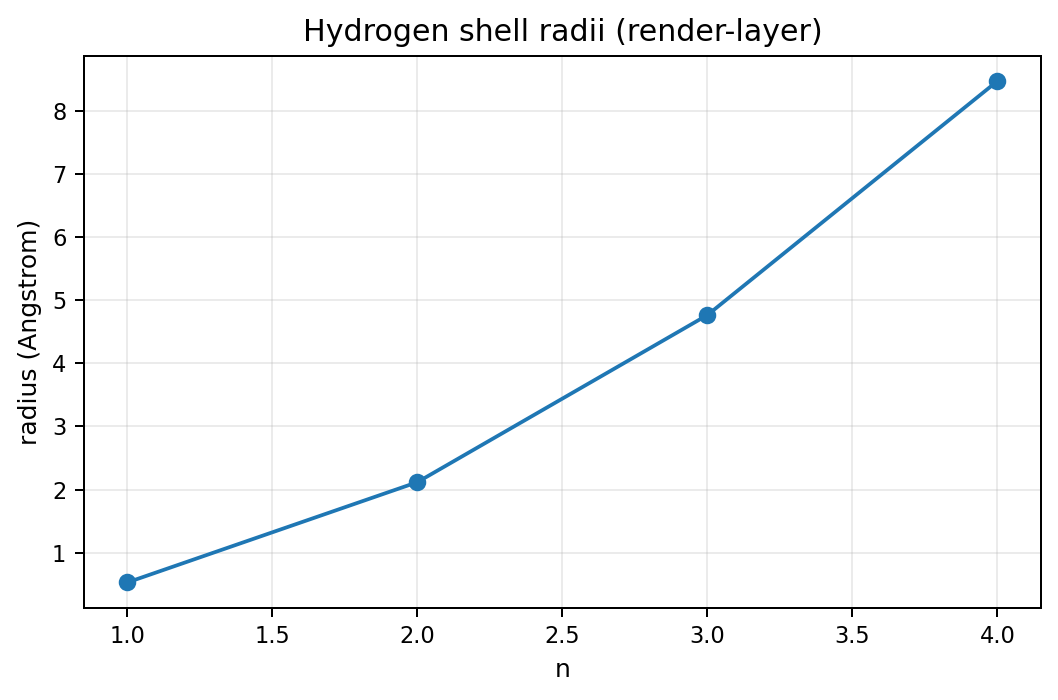
\includegraphics[width=0.74\linewidth]{figures/hydrogen/01_shell_radii.png}
\caption{Hydrogen shell radii attached after the cited shell row is fixed. The plotted radii are report-layer witnesses only; the cited row remains authoritative.}
\end{figure}

\FloatBarrier

\paragraph{Hook / Evidence.}
Use the shell-band and attenuation hooks from the main note together with the local shell report declared in this section.

\subsection{Shell-scale notes}
\label{man:hydrogen-shell-notes}

\paragraph{Readout.}
Shell-facing report algebra remains local to this chapter. It does not alter the naming contract and it does not introduce new theorem content into the main note.
